%pdflatex main.tex
\documentclass[12pt]{article}
\usepackage{natbib}
\usepackage[francais]{babel}
\usepackage{natbib}
\usepackage{url}
\usepackage[utf8x]{inputenc}
\usepackage{amsmath}
\usepackage{graphicx}
\usepackage{float}
\graphicspath{{images/}}
\usepackage{amsthm}
\usepackage{parskip}
\usepackage{fancyhdr}
\usepackage{xfrac}
\usepackage{esvect}
\usepackage{vmargin}
\usepackage{gensymb}
\setmarginsrb{3 cm}{2.5 cm}{3 cm}{2.5 cm}{1 cm}{1.5 cm}{1 cm}{1.5 cm}

\title{POC}								% Title
\author{}								% Author
\date{\today}											% Date

\makeatletter
\let\thetitle\@title
\let\theauthor\@author
\let\thedate\@date
\makeatother

\pagestyle{fancy}
\fancyhf{}
\rhead{\theauthor}
\lhead{\thetitle}
\cfoot{\thepage}
\newtheorem*{rappel}{Rappel}
\newtheorem*{nota}{N.B}
\newtheorem*{req}{Remarque}
\begin{document}

%%%%%%%%%%%%%%%%%%%%%%%%%%%%%%%%%%%%%%%%%%%%%%%%%%%%%%%%%%%%%%%%%%%%%%%%%%%%%%%%%%%%%%%%%

\begin{titlepage}
	\centering
    \vspace*{0.5 cm}
    
\includegraphics[scale = 0.75 ]{logo1.png}\\[1.0 cm]	% University Logo
    \textsc{\LARGE EISTI}\\[2.0 cm]			% University Name
    \rule{\linewidth}{0.2 mm} \\[0.5 cm]
    { \huge \bfseries \thetitle}\\
    \rule{\linewidth}{0.2 mm} \\[1.5 cm]
	\textsc{\Large Projet Différencié}\\[0.5 cm]	% Course Code
	\textsc{\large ING1 GI}\\[0.5 cm]		% Course Name
	
	\begin{minipage}{0.4\textwidth}
	\centering
		\begin{center} \large
		Thomas PIZZINATO \\
		Olivier LISANDRE \\
		Ismaël L'HOSTE \\
		David RIGAUX \\
			\end{center}
			\end{minipage}~
			\begin{minipage}{0.4\textwidth}
	\end{minipage}\\[0.8 cm]
	{\large \thedate}\\[1 cm]
	\vfill
	
\end{titlepage}

%%%%%%%%%%%%%%%%%%%%%%%%%%%%%%%%%%%%%%%%%%%%%%%%%%%%%%%%%%%%%%%%%%%%%%%%%%%%%%%%%%%%%%%%%

\tableofcontents
\addtocontents{toc}{~\hfill\textbf{Page}\par}
\pagebreak

%%%%%%%%%%%%%%%%%%%%%%%%%%%%%%%%%%%%%%%%%%%%%%%%%%%%%%%%%%%%%%%%%%%%%%%%%%%%%%%%%%%%%%%%%

\section{Introduction}
\section{Python}
\section{Réalisation et Résultat}
Pour mener à bien ce projet nous devions découvrir le langage Python ainsi que la façon de l'utiliser pour le dévevelopement web. Nous nous sommes basés sur un formulaire tout simple qui envoyé des informations à l'aide de la méthode \textit{GET} et avons ajoutés petit à petit des fonctionnalitées. Nous avon donc ajouté une base de données statiques et grace à Python nous pouvions manipuler les données dans ce fichier là (\textit{db}). Au final, nous avons décidé d'opter pour la méthode de transfert de données \textit{POST} qui nous permettait d'avoir plus de sécurité quant à l'unicité des données et l'intégrité de celle-ci. Nous nous sommes aidés de Bootstrap pour le style et le javascript, ce qui rend le projet un minimum plus beau visuellement. \br
Voici le résultat :
\begin{figure}[H]
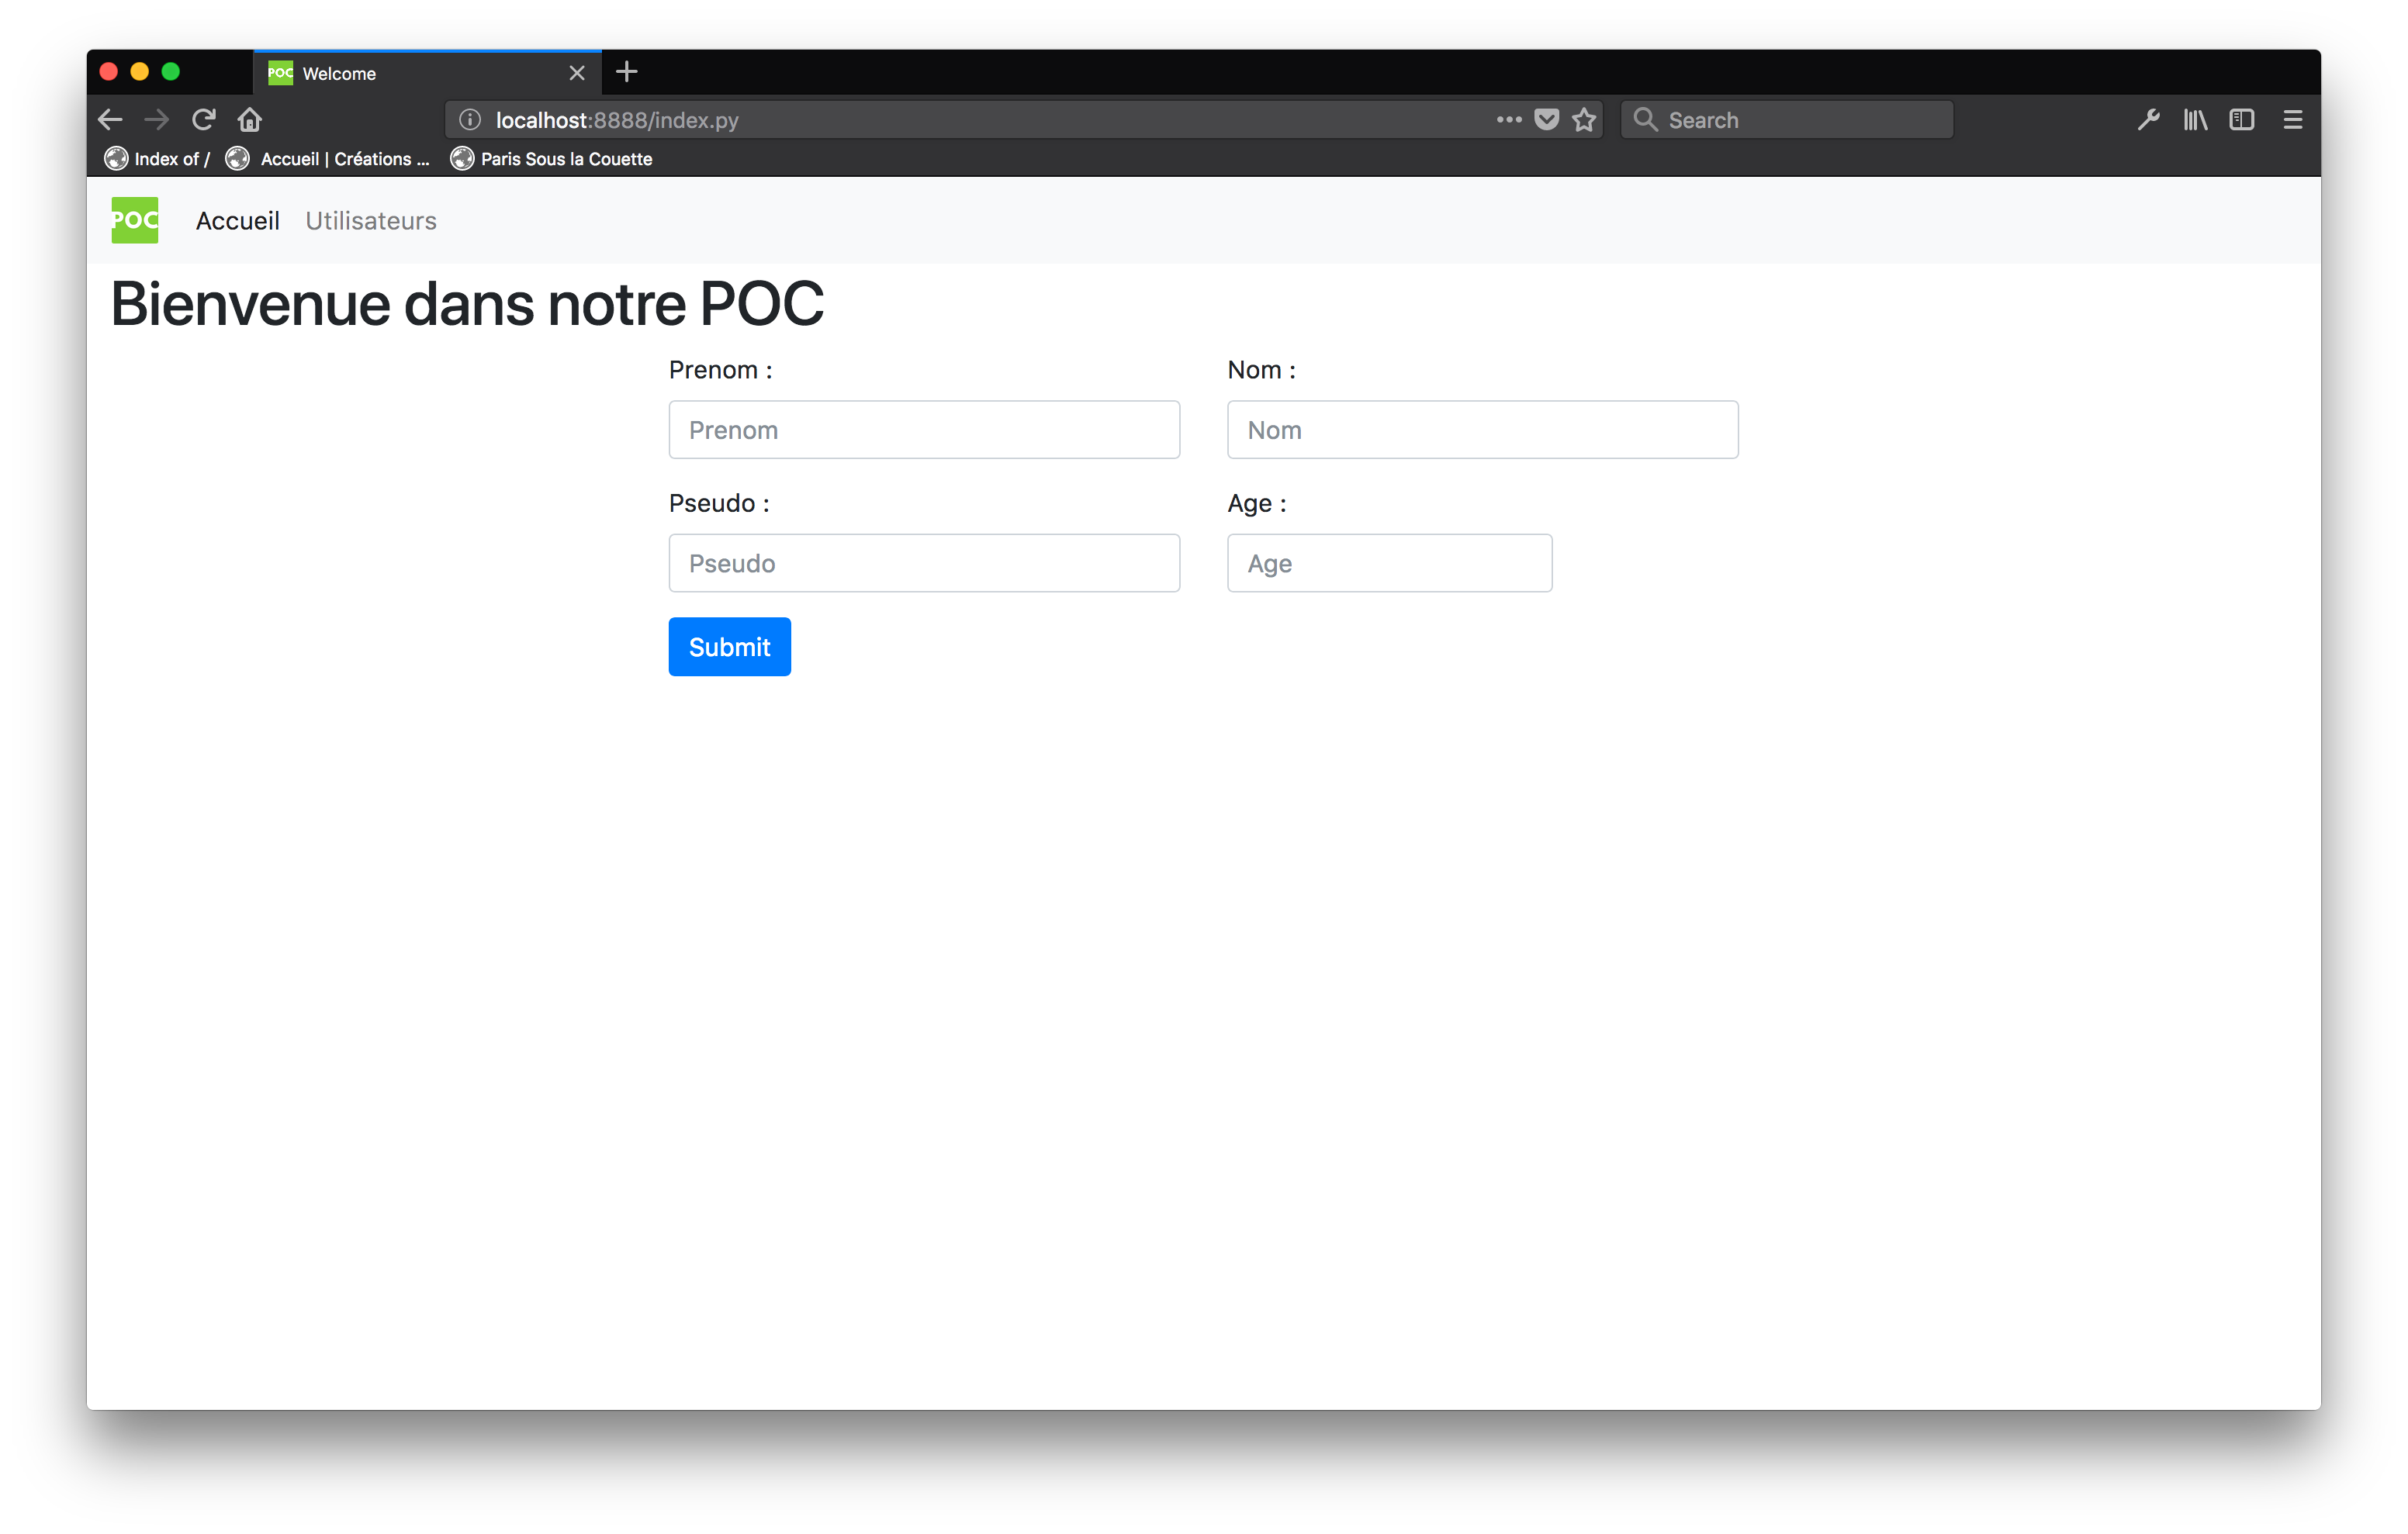
\includegraphics[width=8cm]{images/index.png}
\centering
\end{figure}
\begin{figure}[H]
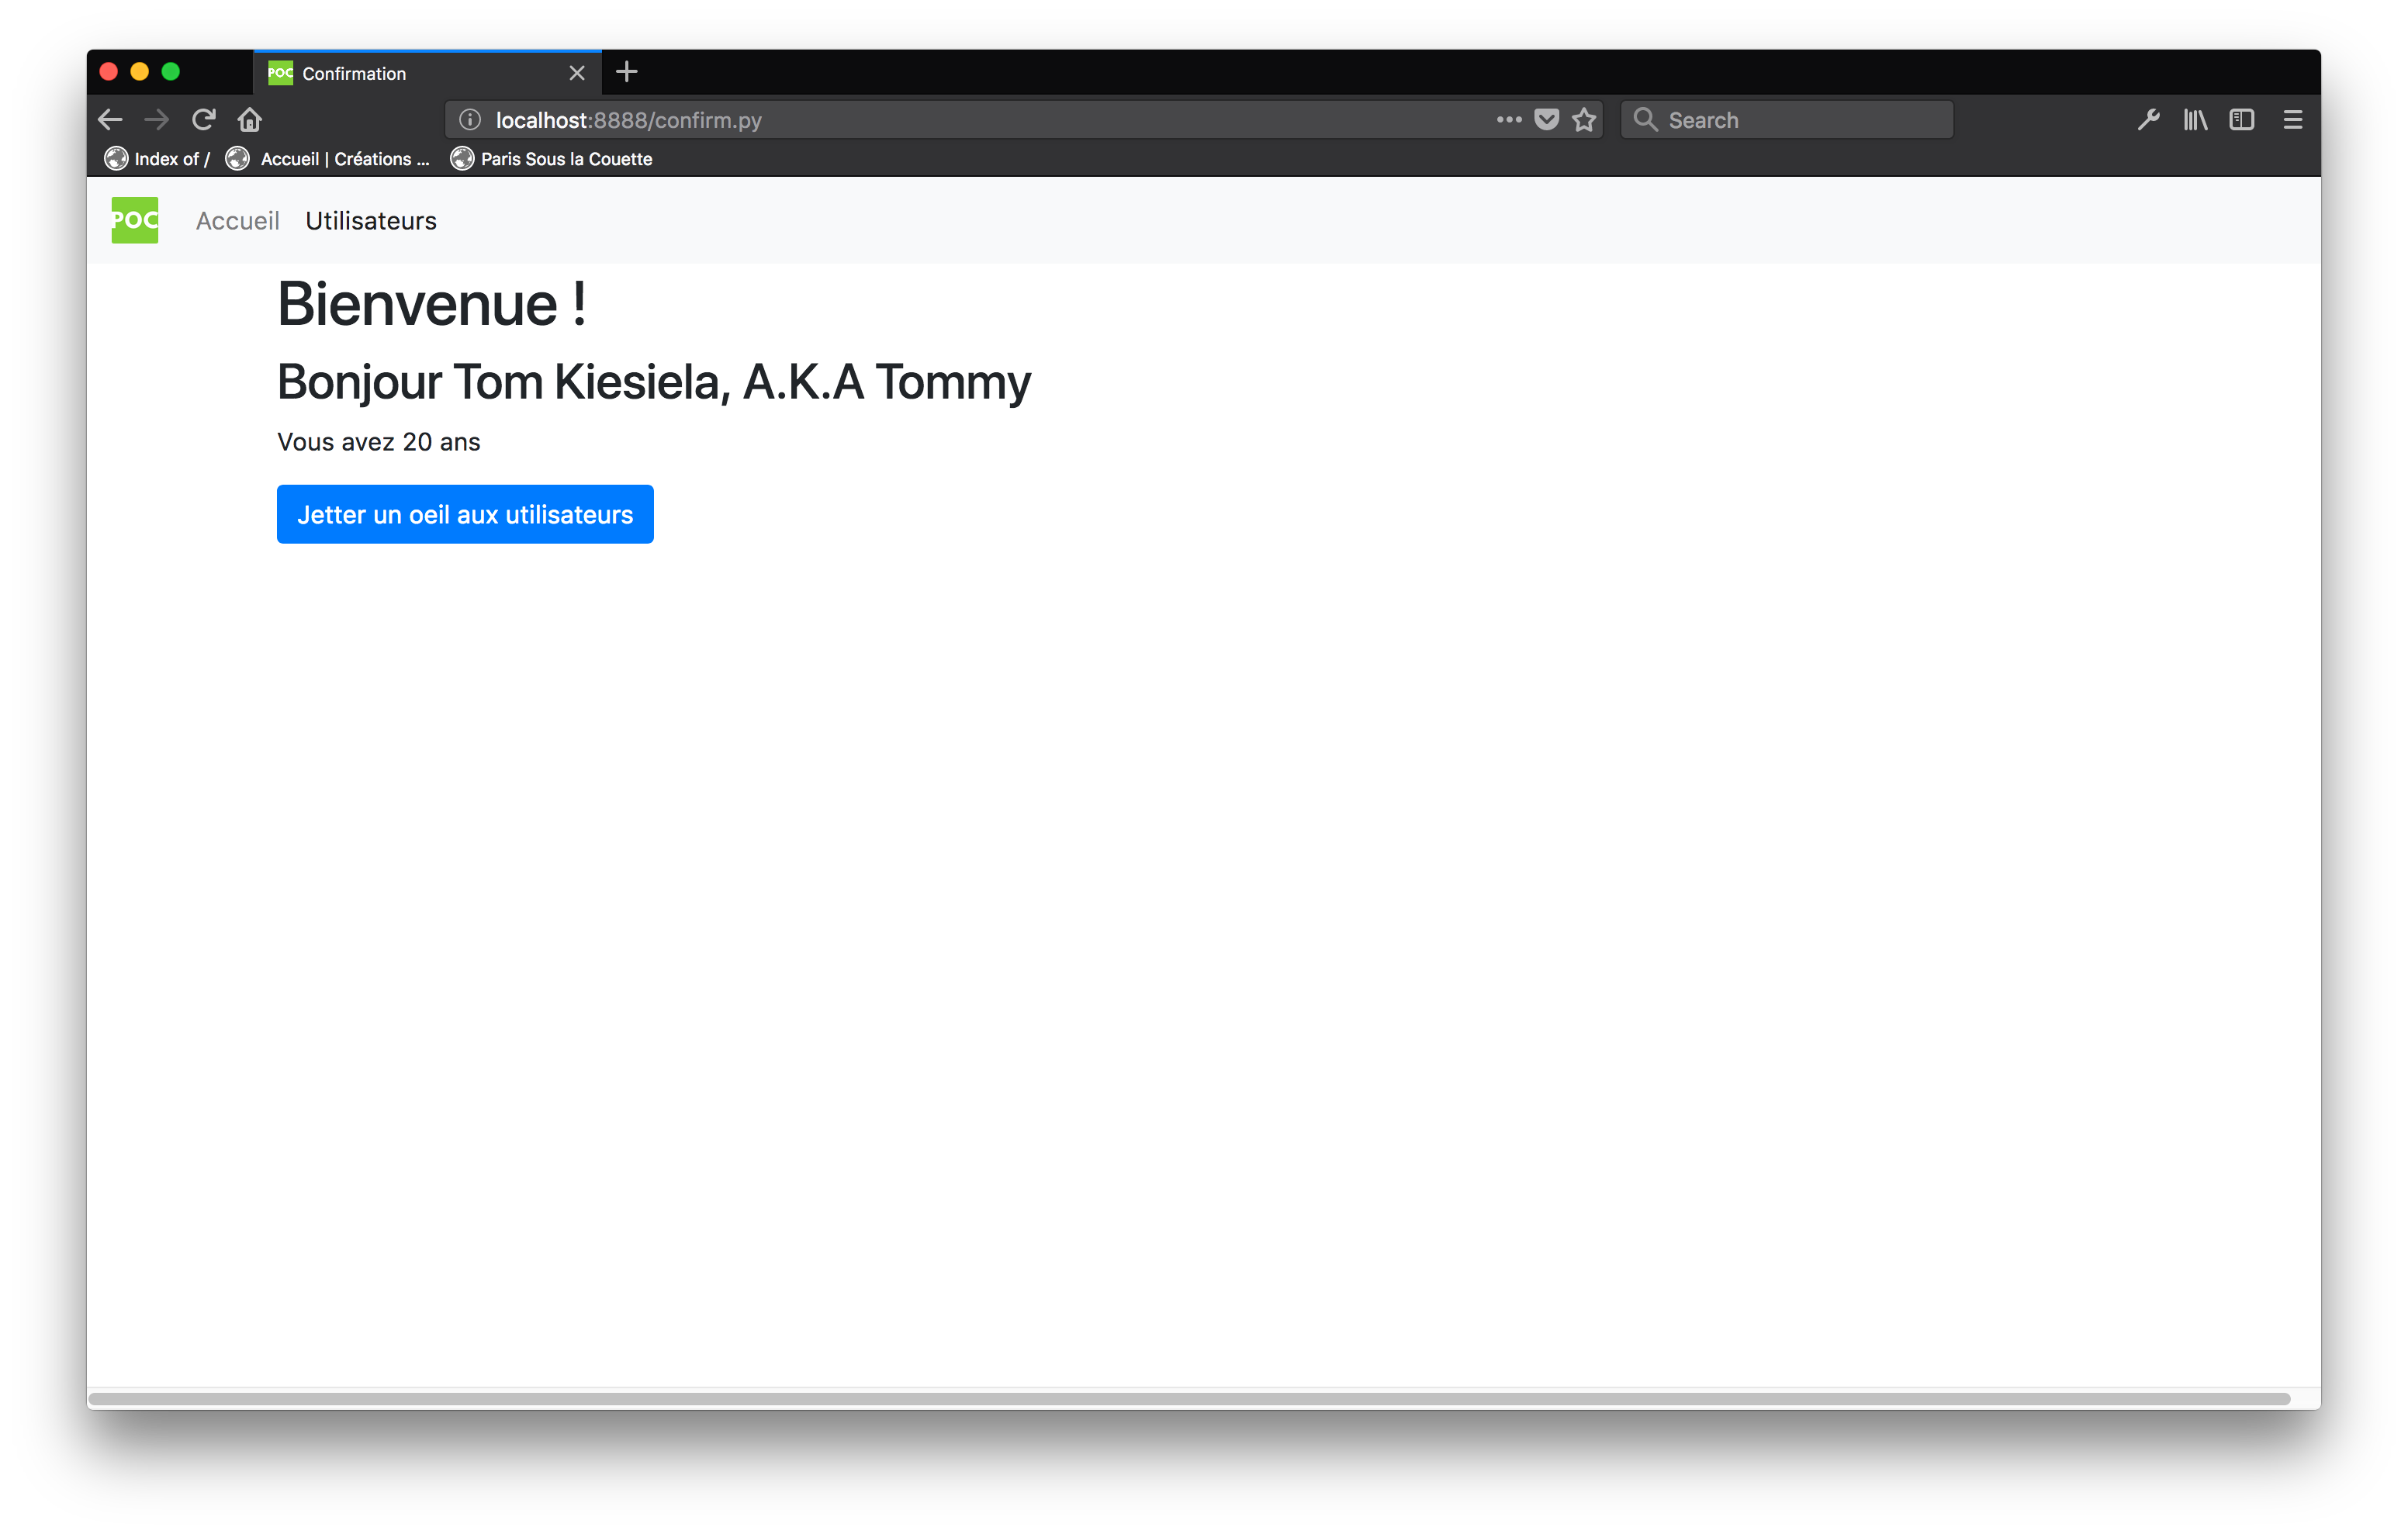
\includegraphics[width=8cm]{images/confirm.png}
\centering
\end{figure}
\begin{figure}[H]
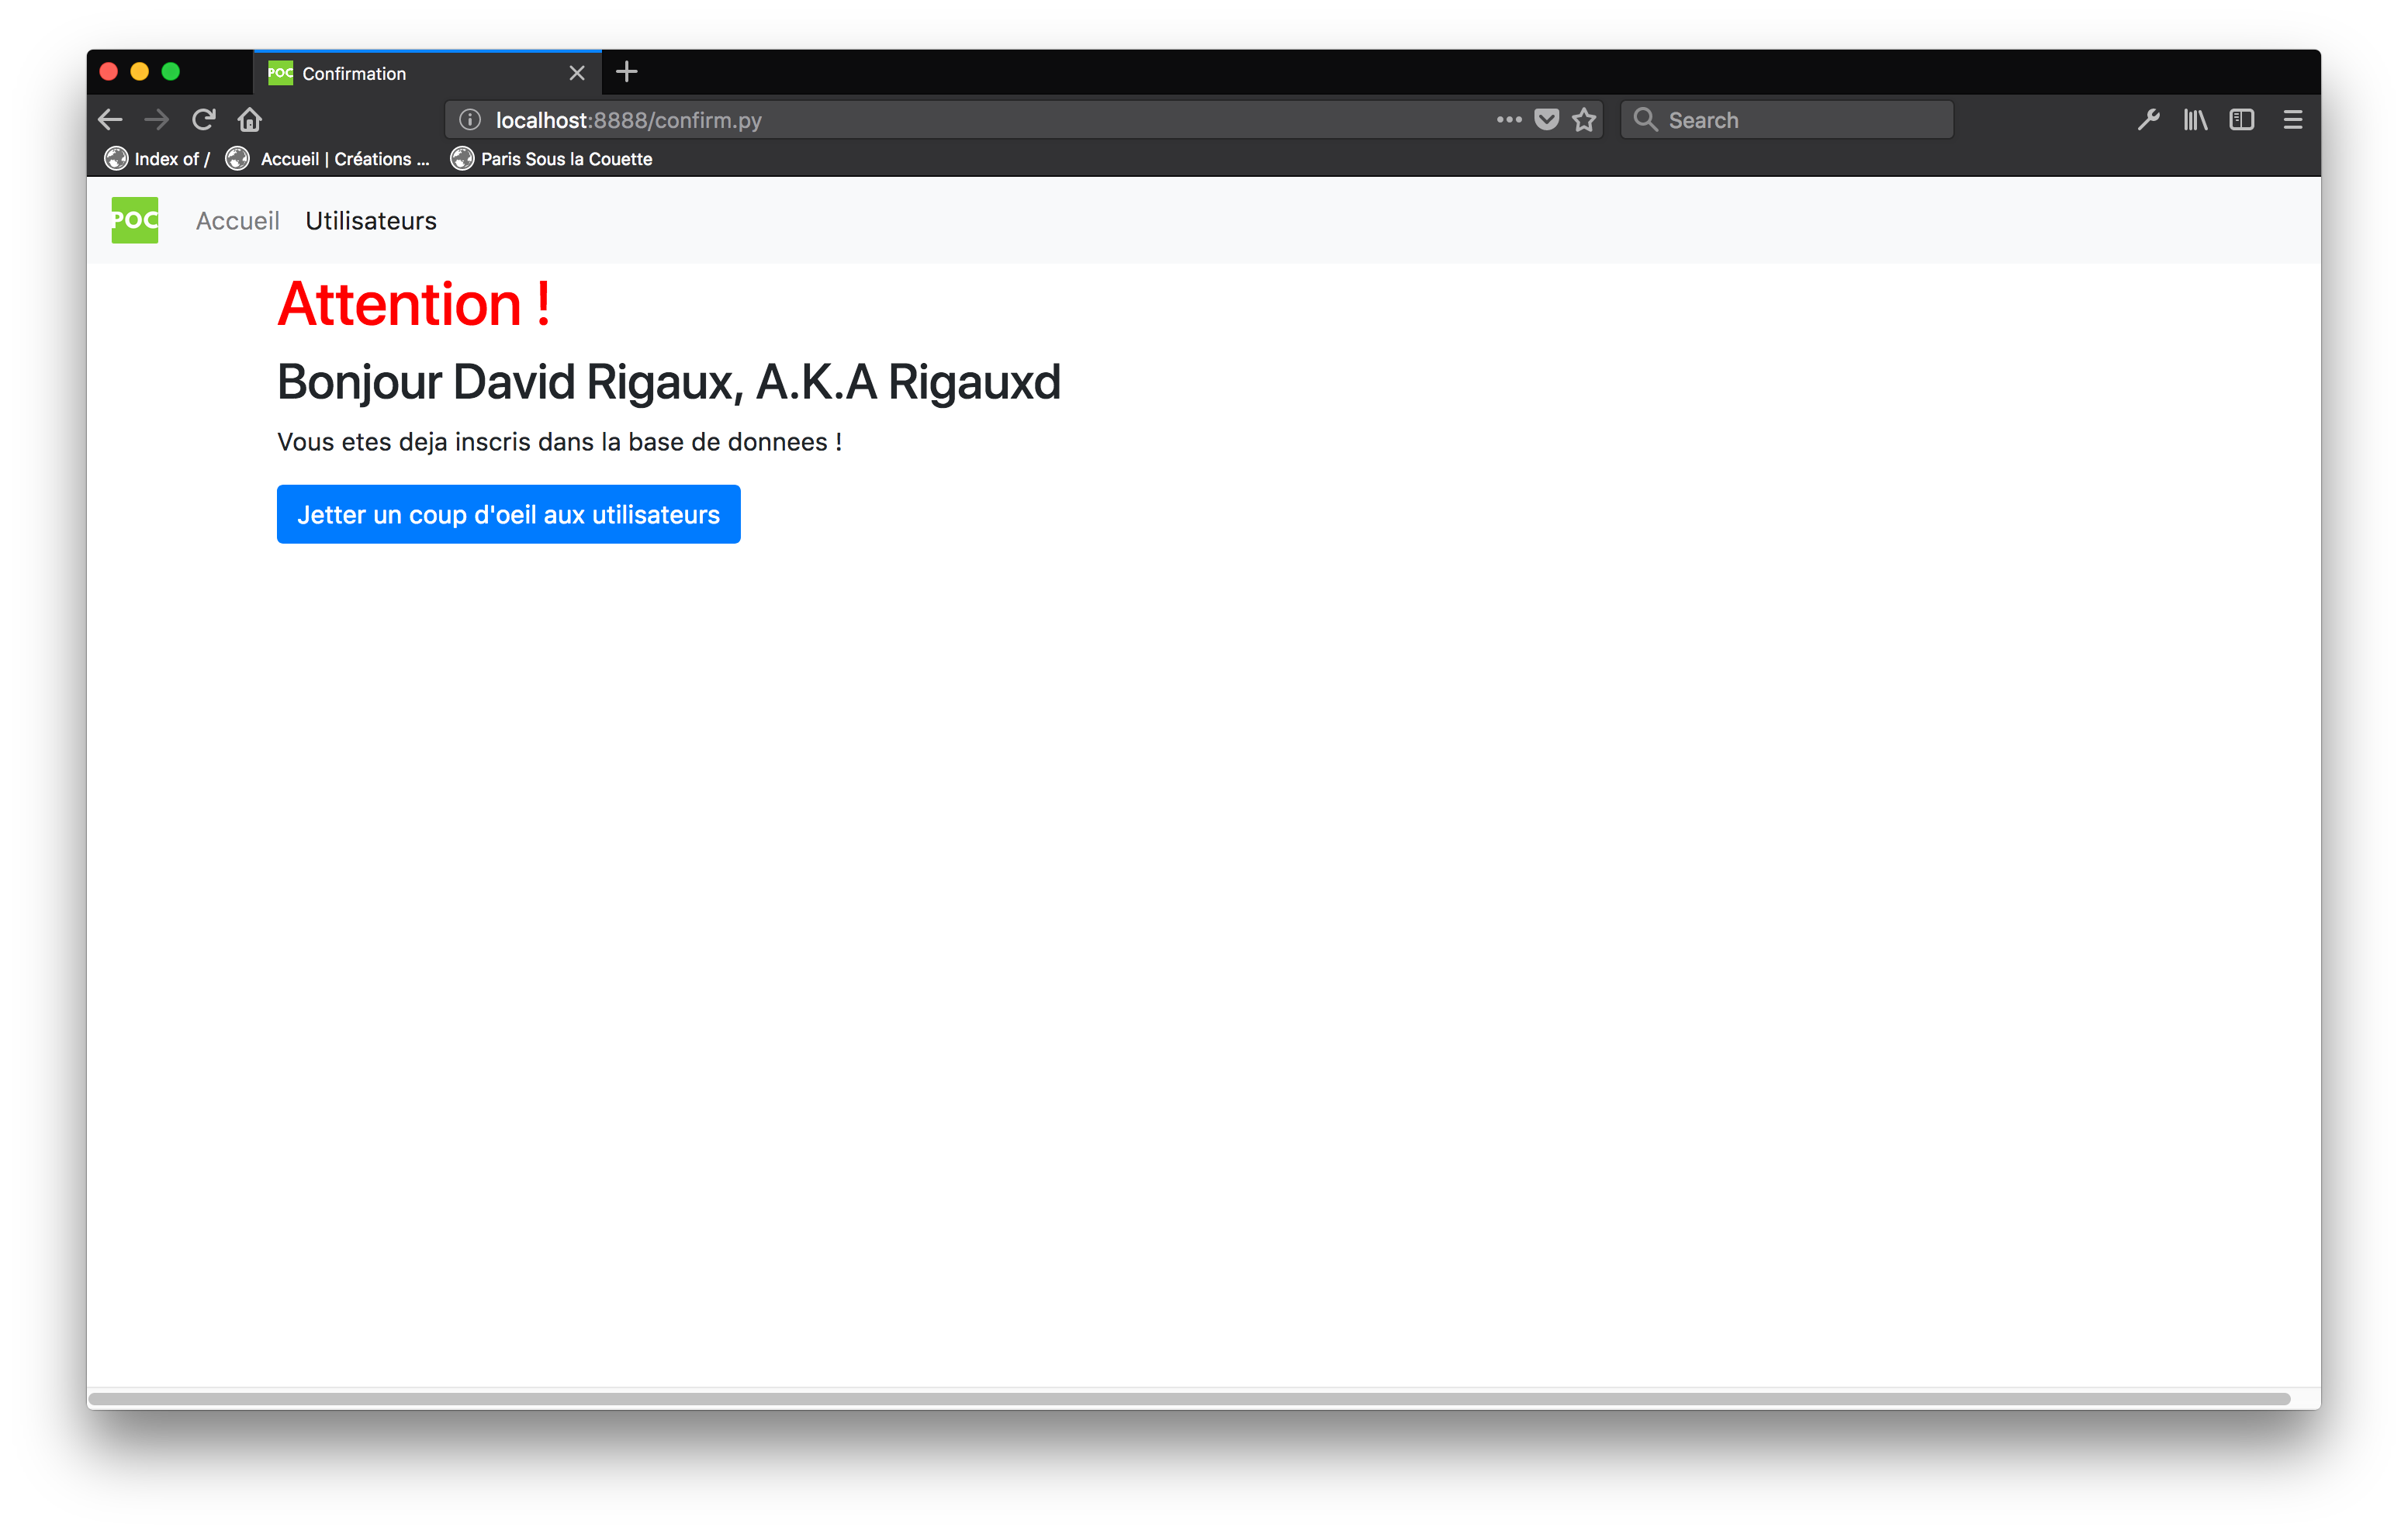
\includegraphics[width=8cm]{images/nonValide.png}
\centering
\end{figure}
\begin{figure}[H]
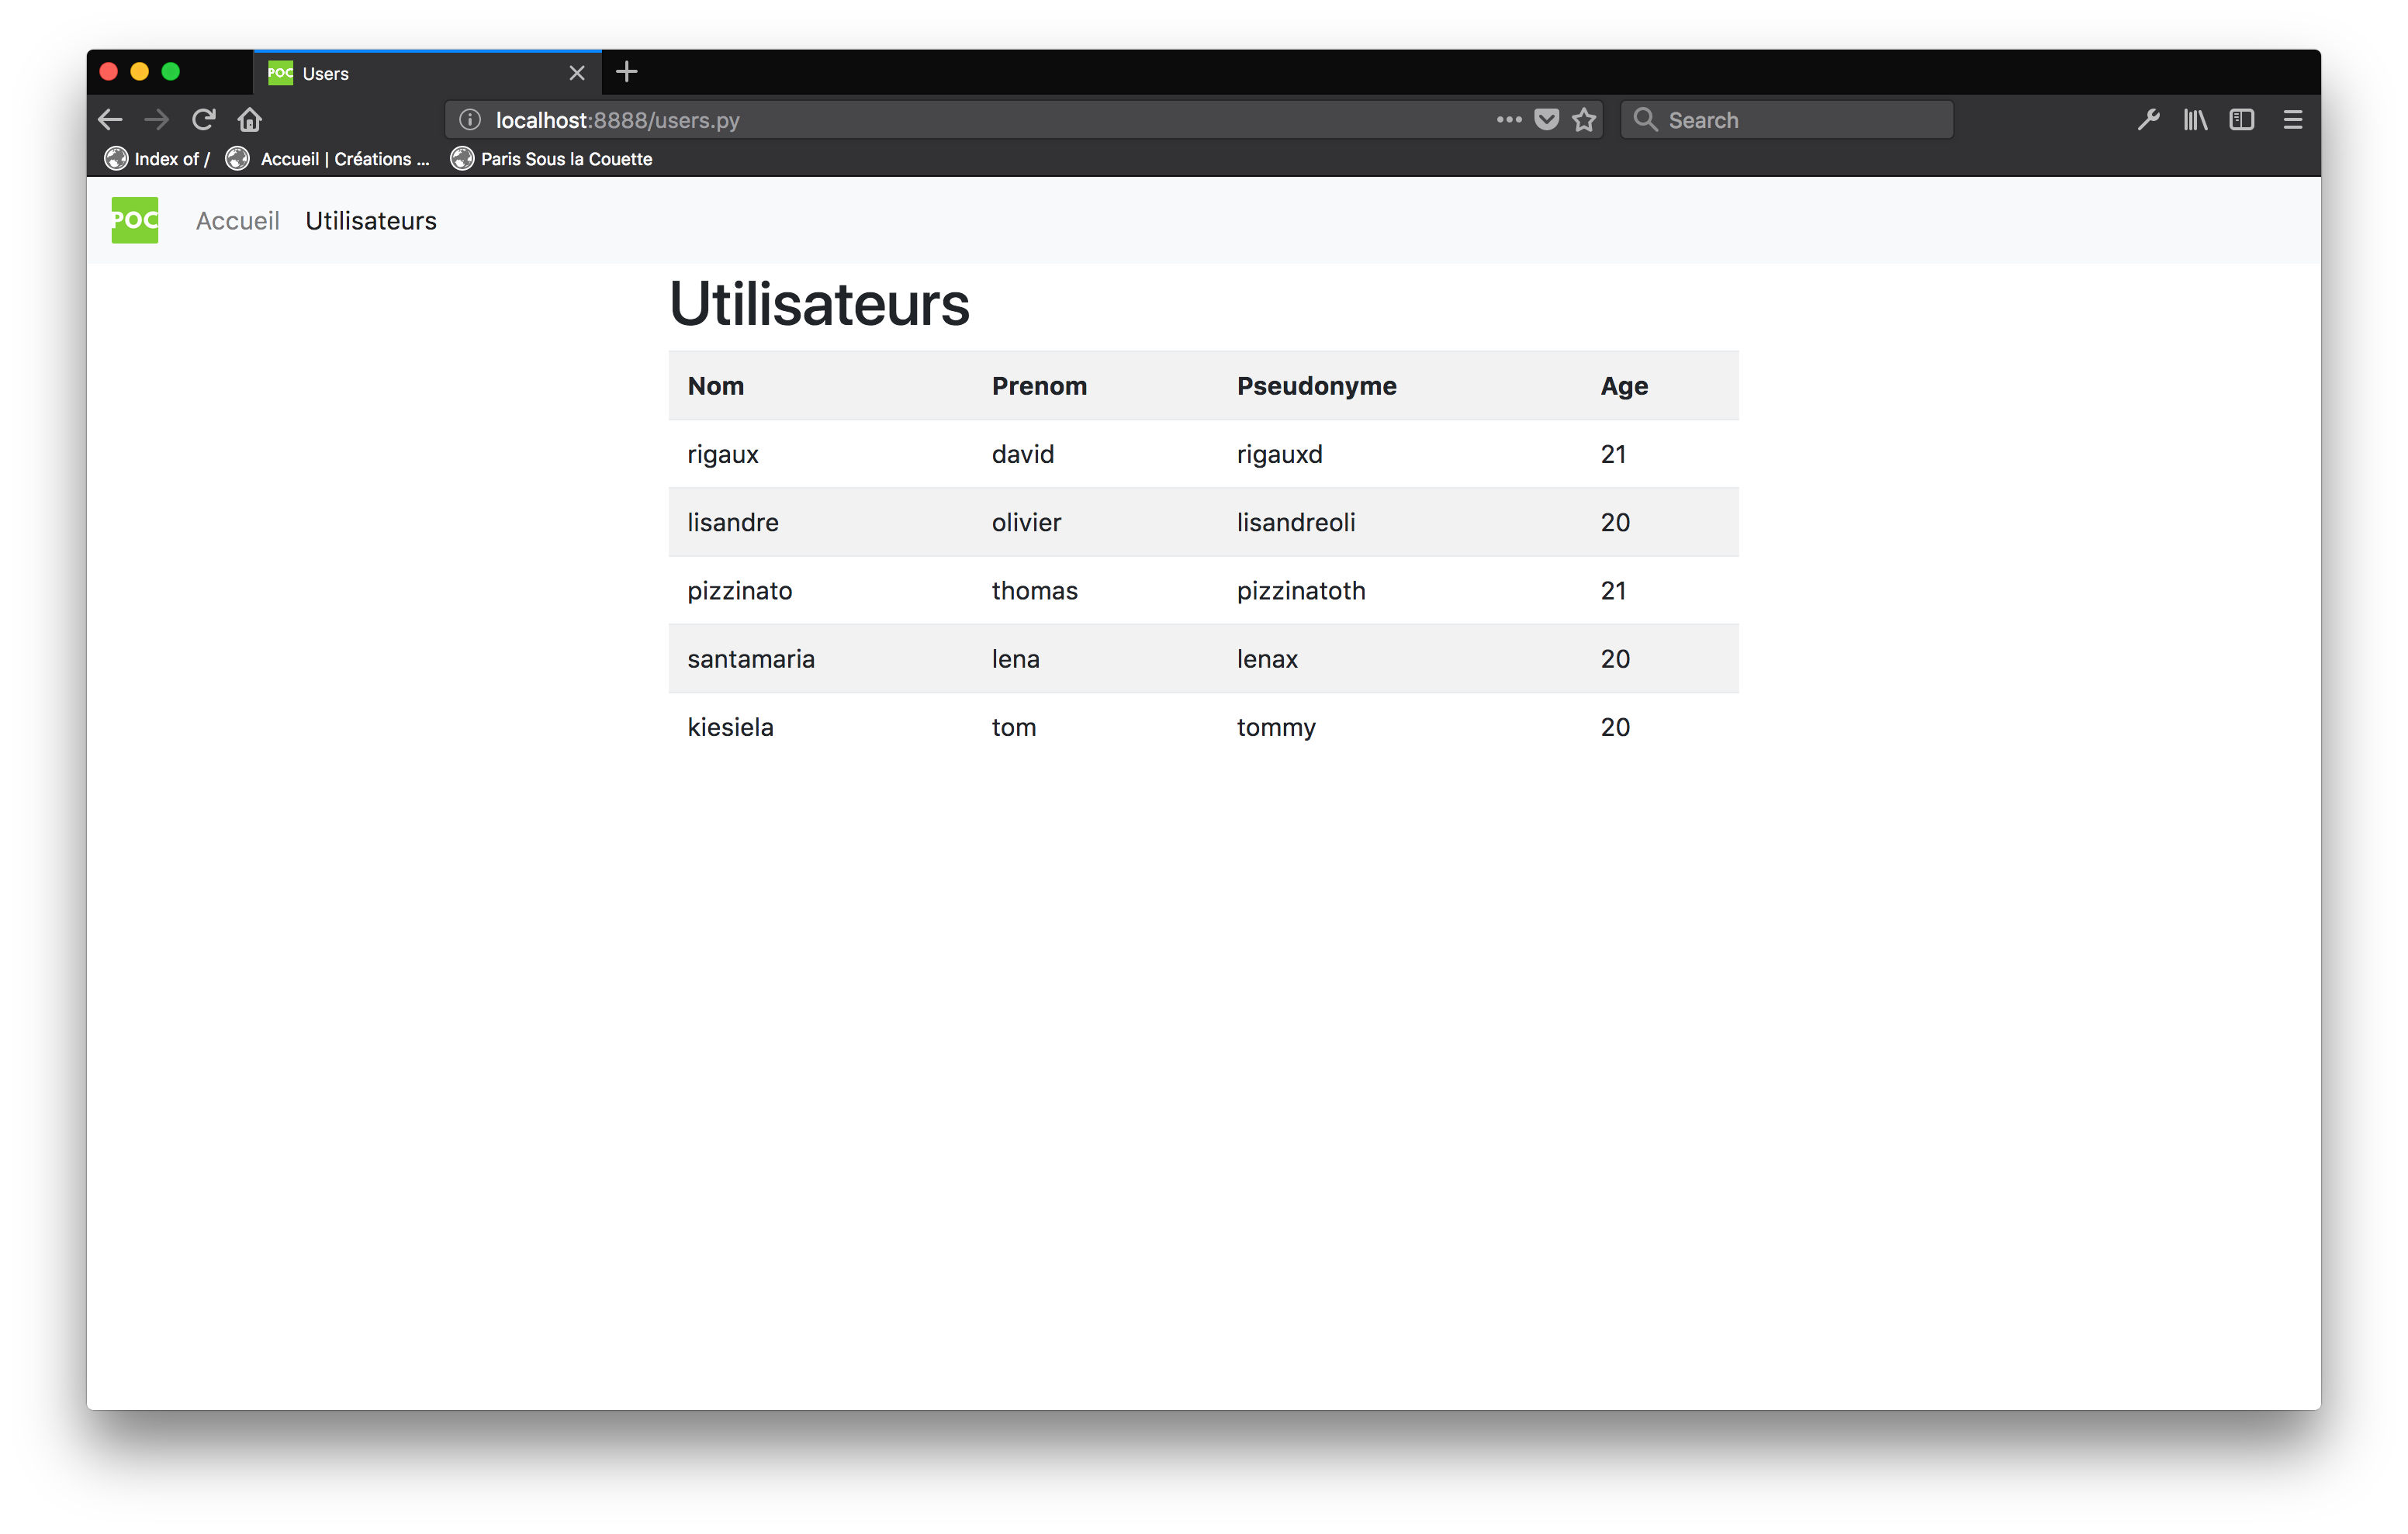
\includegraphics[width=8cm]{images/users.png}
\centering
\end{figure}
\section{Bilan Personnels}
\section{Conclusion}

\end{document}
